%\documentclass[../Manuscrit.tex]{subfiles}
\documentclass[../eBook.tex]{subfiles}

\begin{document}
  \phantomsection
  \addchapterline{Origine de Sermaise -- Etymologie -- Anciennes formes du nom}
  \subsection*{Origine de Sermaise --- Etymologie --- Anciennes formes du nom}
    \paragraph{}L'origine de Sermaise est inconnue, c'est-à-dire qu'il n'existe aucun document faisant connaître l'époque où son territoire a été occupé et mis en culture, où ses premières habitations ont été construites.
    \paragraph{}Si l'on ne sait rien de précis sur l'origine de Sermaise, il faut remarquer que le nom n'a rien de moderne. Il en est de même de Montflix (Mont felix -- heureux), la Rachée, hameaux, \& aussi de S\up{t}-Chéron, Jouy, Dourdan, communes voisines. Enfin on a trouvé dans la vallée d'Orge quantité d'objets antiques qui attestent que cette vallée est habitée depuis longtemps. C'est ainsi que les jolis pavages mosaïques découverts à S\up{te}-Mesne marquent l'emplacement d'une somptueuse villa gallo-romaine. À Saint-Evroult de la commune de Saint-Chéron, une chaussée et des aqueducs mis à jour rappellent aussi les temps gallo-romains.
    \paragraph{}A Souzy, situé à 5 kilomètres, des mosaïques de la même origine ont été déterrées et enlevées vers 1868. Dans cette même localité, on a découvert des roches en grès qui ont dû servir à polir et à aiguiser des outils et des instruments en pierre. L'une de ces roches ne contient qu'une seule rainure, mais l'autre en porte neuf, dont sept à côté l'une de l'autre et parallèles permettaient sans doute de polir plusieurs instruments à la fois.
    \paragraph{}Je dois ajouter que des fragments de haches en silex ont été trouvés sur notre territoire et semblent ici une trace de l'âge de la pierre. Quelques-uns de ces fragments sont déposés au musée scolaire.
    \paragraph{}Cependant, si l'on jette un coup d'\oe il à travers ce vaste territoire, on découvre des restes d'habitations anciennes : à Blancheface (Château Gaillard), entre le Mesnil \& la Rachée (Clos Goury), à Montflix (les trois murgers), dans la plaine du Tertre, au pied de la butte du même nom, à Haute-Minière et aussi dans les pentes de la Bretonnière et de la Duboiserie. Ces constructions étaient isolées. Il est vrai que les ancêtres aimaient peu le voisinage : chacun d'eux s'établissait près d'une fontaine ou d'un cours d'eau, dans une campagne ou dans une forêt où il se logeait avec sa famille au milieu des terres qu'il cultivait. La première idée de Patrie, le besoin fréquent de s'unir contre l'ennemi commun, les premières lueurs de l'instruction, et aussi le désir du bien-être par le progrès, ont peu à peu rapproché les hommes et formé la société actuelle, éclairée, hospitalière, forte et confiante dans l'avenir.

    \vspace{12pt}
    \noindent\dotfill
    \paragraph{}Sermaise doit peut-être son nom à la disposition de ses coteaux en circuit, et entre lesquels se trouvent groupés en \underline{cercle} les \underline{maisons} du village. Quelques-uns prétendent, à tort ou à raison, que Sermaise a été fondé par une colonie de Sarmates établie ici lors des invasions ; mais il faut remarquer que plusieurs communes de France portent le même nom et aussi que les Sarmates, après avoir pris part à l'invasion des Huns en Gaule, se sont établis sur les bords de la Baltique.
    \paragraph{}L'orthographe du mot a eu différentes formes. Il y avait au 15\up{e} siècle un baron de Sergmès ; sur les actes de l'état civil on dit d'abord \og \textit{Sermaises} \fg{} au 17\up{e} siècle, puis \og \textit{Sermaize} \fg{} et enfin \og \textit{Sermaise} \fg{} à partir de 1780. Dans un guide très ancien sur les environs de Paris on voit : Sarmaize, village sur la route de Dourdan, 11 lieues.

  \phantomsection
  \addchapterline{Sermaise sous l'ancien régime}
  \subsection*{Sermaise sous l'ancien régime}
    \paragraph{}Au temps de la \underline{féodalité}, Sermaise était le siège d'un grand nombre de fiefs plus ou moins importants \& dépendant de seigneurs différents.
    \paragraph{}Il y avait les fiefs de Villeneuve, de Mondétour (Maudestour), de la Grange de Maugrenoult, de Montflix, du Mesnil, de la Rachée, de Trousse-Chien. Le Tertre faisait partie du domaine du Marais. Un lieu-dit de Sermaise, le bois de Graville, tire son nom des seigneurs de Graville, barons de Saint-Yon.
    \paragraph{}La seigneurie de la paroisse relevait de celle de Milly, en Gâtinais ; elle a été possédée depuis le XIV\up{e} siècle, au moins, jusque dans le XVIII\up{e} par la famille Descrosnes \& par celle de Hémery qui lui a succédé par alliance. François de Hémery en a fait la vente en 1733 à G. de Lamoignon qui par un traité de 1735 en est resté seul propriétaire ainsi que des droits de pêche, de chasse, de patronage de la Chapelle-S\up{t}-Georges.
    \paragraph{}Anne d'Autriche, mère de Louis XIV, avait détaché Sermaise du comté de Dourdan en faveur de Guillaume de Lamoignon, premier président de la cour du parlement, seigneur de Saint-Chéron, Bâville etc. Les officiers du bailliage de Dourdan, qui perdaient quelque chose à cet amoindrissement du ressort furent dédommagés d'un autre côté. Le premier président de Lamoignon donna comme indemnité à M. Vedye, lieutenant général au bailliage la charge \& office de prévôt de Dourdan, et aux autres officiers du bailliage les diverses commissions de la prévôtée.

    \phantomsection
    \addsectionline{Justice \& tabellionage}
    \subsubsection*{Justice \& tabellionage\footnote{\textit{NDLR} --- Synonyme de notariat}}
      \paragraph{}A l'égard de la haute justice, Sermaise dépendait du Comté royal de Dourdan et il en était de même du tabellionage. Ces deux droits seigneuriaux ont été donnés en 1661 par la reine mère à Guillaume de Lamoignon qui les a fait entrer dans son marquisat de Bâville. Antérieurement, Sermaise a été la résidence d'un substitut juré ou d'un sous fermier de tabellionage de Dourdan, en d'autres termes, une des branches de ce tabellionage.
      \paragraph{}Parmi ces fonctionnaires il faut citer Etienne Bedeau qui se qualifiait de substitut juré, commis au lieu \& paroisse de Sermaise, d'abord sous Jean Perrier, tabellion à Dourdan, en 1537, et ensuite sous Marin Deschamps tabellion royal à Dourdan, de 1538 à 1570. Pendant l'exercice d'Etienne Bedeau, il y avait encore un substitut à Montflix, paroisse de Sermaises comme l'atteste le titre suivant que nous copions tout simplement :
      \begin{quote}
        \og \textit{Censier reçu par noble homme M\up{e} Pierre Chartier, seigneur du Tartre (Tertre) et de Baudrecourt, notaire \& secrétaire du roi \& greffier en sa chambre des comptes, en son hostel seigneurial du Tartre, Paroisse de Sermaises, bailly de Dourdan , en la présence de moy, Claude Bailly, substitut au lieu de Montflix pour Jehan Pesan, tabellion à Dourdan}. \fg{}
      \end{quote}
      \paragraph{}Citons encore comme tabellions : Jean Thiboust (1557) ; Pierre Descoutures  (1559) ; Jean Le Cousturier de 1576 à 1613, à Blancheface ; Jean de Narenne, de 1585 à 1588, à Sermaise ; Georges Le Cousturier, sans doute frère de Jean Le Cousturier, de 1613 à 1622, à Blancheface ; Simon Le Cousturier, de 1614 à 1642 ; Jean Coudray, 1639 ; Jean Houdouin, de 1648 à 1670 ; Pierre Besnard, de 1670 à 1701. Pierre Besnard est devenu seul tabellion à Sermaises à partir du jour où a cessé l'exercice de Jean Houdouin. En 1673 il était greffier à Bâville, et paraît avoir conservé ces fonctions jusqu'en 1692. En 1680 il a exercé les fonctions de bailli pour cause d'absence de celui-ci.
      \paragraph{}En 1692 on le trouve procureur fiscal du bailliage de Bâville. Outre ces fonctions, Pierre Besnard était fermier conjointement avec son frère, Jean Besnard, des droits de greffe \& de tabellionage des paroisses de Sermaises et Saint-Chéron ; mais en 1701 Pierre Besnard quoique se disant tabellion de Sermaises demeurait à Saint-Chéron. A partir de cette époque, la résidence d'un notaire à Sermaises a cessé et le droit de tabellionage a toujours été exercé par le tabellion de Saint-Chéron.
      \paragraph{}Sermaise ne paraît pas avoir été depuis le 15\up{e} siècle en possession d'une justice instituée de sorte que les affaires contentieuses qui s'y produisaient devaient être portées au Bailliage de Dourdan dans le ressort duquel elle était. Toutefois il s'y trouvait une résidence de Sergent. Car en 1640 on trouve que Gauldon y était sergent royal. Lorsque cette paroisse fut détachée de Dourdan \& unie au marquisat de Bâville en 1670, la résidence du sergent paraît y avoir persisté jusqu'en 1701. Louis Claude Augé se qualifiait de sergent ordinaire au Bailliage de Bâville, demeurant à la Charpenterie de Sermaises.

  \phantomsection
  \addchapterline{À travers les hameaux et écarts de Sermaise}
  \subsection*{À travers les hameaux et écarts de Sermaise}
    \phantomsection
    \addsectionline{Mondétour}
    \subsubsection*{Mondétour}
      \paragraph{}Mondétour, ou plutôt Maudestour (mauvais détour) a été appelé ainsi à cause de sa situation escarpée et autrefois de ses mauvais chemins sur un sol glaiseux.
      \paragraph{}Les familles Brière \& Mesnard ont ajouté Mondétour à leur nom en le faisant précéder de particule dite nobiliaire. Ainsi Jean Brière, ex-secrétaire du roi Louis XVI, né en 1711, mort en 1798, prend la qualité d'ecuyer sieur de Mondétour en partie. Isidor Simon Brière de Mondétour est ainsi nommé dans le mariage de sa soeur, M\up{me} Buchère, en 1777.
      \paragraph{}François Nicolas Brière ajoutait de Mondétour à son nom dès 1778. Tous ses actes de notaire sont signés Brière de Mondétour et ses enfants ont conservé le même nom, sauf l'un d'eux qui, par décret de 1818, a été autorisé à ajouter Valigny à son nom, et à s'appeler Brière de Mondétour-Valigny.
      \paragraph{}Plusieurs des enfants de Jean Baptiste Mesnard, régisseur à Bâville, ont également pris le nom de Mesnard de Mondétour. Cette addition de nom est fondée principalement sur un contrat de 1733 par lequel Paul Augustin Dubuisson, écuyer, seigneur de Mondonville et Elisabeth Catherine Daverton, sa femme, issue des anciens seigneurs de Blancheface, ont vendu à Etienne Mazure, procureur fiscal du marquisat de Bâville et à Marie-Madelaine Langlois sa femme : \hrulefill
      \begin{quote}
        \og \textit{La ferme de la Guérenardière, située à Mondétour, 38 arpents de terre en dépendant, 50 arpents de terre, prés, bois \& vignes, situés au même lieu, étant en rôture \& charge de cens \& rentes, et 11 livres de rentes constituées en 3 parties.} \fg{}
      \end{quote}
      \paragraph{}L'ancienne ferme existe encore et sous l'Empire la famille Brière a fait construire auprès, en style de l'époque, une confortable maison d'habitation, dite château de Mondétour, entourée d'un parc et habitée aujourd'hui par M. Talabart, avocat.

    \phantomsection
    \addsectionline{La Villeneuve}
    \subsubsection*{La Villeneuve}
      \paragraph{}La Villeneuve a été le théâtre de meurtres atroces commis au siècle dernier par la bande de Renard. C'est pour mémoire que nous dirons quelques mots de cette illustre société de bandits. Extrait d'un arrêt de la Cour du Parlement du 26 février 1766, qui condamne à la peine de mort Jean François Renard, Toussaint Soubriat, Pierre Farneau, Jean Sébastien Cordel, Jean Garnier \& autres :
      \paragraph{}Cet arrêt confirme une sentence rendue le 22 août 1765 par le lieutenant criminel du Bailliage de Dourdan et par laquelle :
      \begin{quote}
        \og \textit{Les dits Jean François Renard, Toussaint Soubriat dit le jardinier de Châtenay, Pierre Farneau dit Baptiste Lapin et Jean Sébastien Cordel dit le soldat, auraient été déclarés dûment atteins \& convaincus d'avoir, avec d'autres de leurs complices de dessein prémédité, commis nuitamment le 26 au 27 décembre 1763 cinq assassinats dans une seule \& même maison, au hameau de Villeneuve, paroisse de Sermaise-sous-Dourdan, ès personnes de Jeanne Perry, veuve de Pierre Rocher, Pierre Canet, vigneron, son gendre et Denise Chevallier leur servante domestique, et encore Louis Malherbe, vigneron demeurant au hameau de Beauvais paroisse de Roinville, et de Pierre Leblanc aussi vigneron demeurant au village de S\up{t}-Chéron Montcouronne qui se sont trouvés dans la dite maison, et ensuite d'avoir volé la plus grande partie des effets, hardes, nippes, toiles, chemises, deniers comptants \& autres, mentionnés au procès, appartenant tant à la dite V\up{ve} Rocher, Pierre Canet son gendre, qu'à la dite Chevallier leur servante domestique.} \dotfill \fg{}
      \end{quote}
      \paragraph{}(suivent un grand nombre d'autres forfaits que nous ne citons pas n'ayant pas un caractère local)
      \begin{quote}
        \og \textit{Pour réparation de quoi les dits Jean François Renard, Toussaint Soubriat dit le jardinier de Châtenay, Pierre Farneau dit Baptiste Lapin, Jean Sébastien Cordel dit le soldat, Jean Garnier dit Breton, et Pierre Louis Antoine Duhamel dit le petit Parisien auraient été condamnés à avoir tous  six les bras, jambes, cuisses \& reins rompus vifs par l'executeur de la haute justice, sur un échafaud qui pour cet effet serait dressé en la principale place de la ville de Dourdan et mis ensuite sur chacun une roue, la face tournée vers le ciel, pour y demeurer tant et si longuement qu'il plaira à Dieu leur conserver la vie ; ce fait, leurs corps morts portés par l'exécuteur de la haute justice, savoir : ceux des dits Renard, Soubriat, Farneau \& Cordel sur le grand chemin de la dite ville de Dourdan à Sermaise, et à l'endroit en face dudit hameau de Villeneuve, où cinq personnes ont été par eux assassinées.} \fg{}
      \end{quote}
      \paragraph{}Un complice, Antoine Charron dit tourne talon, condamné par le même arrêt a être pendu fut également exposé après sa mort sur la route de Dourdan en face de Villeneuve.
      \begin{center}
        \begin{figure}[!ht]
          \ifthenelse{\equal{\colorspace}{CMYK}}{\includegraphics[width=\textwidth]{CMYK/03-his-01-villeneuve.jpg}}{\includegraphics[width=\textwidth]{RGB/03-his-01-villeneuve.jpg}}
          \caption*{Vue sur la route de Dourdan (prise du Tertre)}
        \end{figure}
      \end{center}
      \small{}
      \noindent\textbf{1.} Hauteurs de Villeneuve où se trouvait au siècle dernier une maison isolée dont on voit encore quelques vestiges et qui fut le théâtre des meurtres cités.\\
      \textbf{2.} Route de Dourdan où ont été exposés les cadavres des bandits Renard, Soubriat, Farneau, Cordel \& Antoine Charron dit tourne talon.
      \normalsize{}
      \paragraph{}Après le supplice de Renard et de 31 de ses compagnons, le reste de la bande émigra dans la forêt de Montargis en chantant : \og \textit{Dedans Dourdan ils sont méchants ...} \fg{}.
      \paragraph{}Les crimes atroces recommencèrent, et le fameux Robillard, le nouveau chef, pris \& condamné par jugement prévôtal de Montargis, paya sa dette envers la justice le 13 septembre 1783 avec soixante-dix autres brigands de sa société qui se partagèrent la roue, le gibet\footnote{\textit{NDLR} --- Potence pour les condamnés à la pendaison} et les galères.
      \paragraph{}La bande d'Orgères, comme on l'appelait n'était pas entièrement détruite : Fleur d'Epine, issu de Renard la reconstitua plus terrible que jamais.
      \paragraph{}Ces parias du crime, avec leurs m\oe urs étranges, leur code barbare, leurs mariages sommaires, leurs rites immondes \& leurs parodies sociales s'étaient alors cantonnés dans les bois de Saint-Escobille et exploitaient les vastes espaces et les hameaux écartés de la Beauce.
      \paragraph{}Connus \& redoutés sous le nom de \og \textit{Chauffeurs} \fg{}  parce qu'ils brûlaient lentement les pieds de leurs victimes pour obtenir des révelations de trésors, ils ne s'inquiétaient pas si la Révolution avait changé les bases de la société, et, terroristes indépendants, ils suivaient la fortune du Rouge d'Aneau \& de ses satellites.
      \paragraph{}Le siècle, en commençant, finit leur histoire et les 12 vendémiaire an IX (30 octobre 1800), la guillotine de Chartres dévora coup sur coup les 21 têtes des derniers chefs.
      \paragraph{}Ces brigands du siècle passé sont déjà légendaires, et le roman s'est emparé de cette chronique sinistre dont Dourdan \& les environs peuvent fournir le premier \& le plus émouvant chapitre.

    \phantomsection
    \addsectionline{Bellenger}
    \subsubsection*{Bellenger}
      \paragraph{}Bellenger, originairement appelé le Petit-Moulin, aujourd'hui non exploité, vient d'une famille très ancienne.
      \paragraph{}Son nom se trouve déjà dans des titres de 1295, écrit \og \textit{Bérangier} \fg{} ; en 1376 il est encore orthographié de même ; en 1510 il devient Bellenger, et en 1757 il est encore représenté par Jean Bellenger des environs de S\up{t}-Chéron.
      \begin{center}
        \begin{figure}[!ht]
          \ifthenelse{\equal{\colorspace}{CMYK}}{\includegraphics[width=\textwidth]{CMYK/03-his-02-bellenger.jpg}}{\includegraphics[width=\textwidth]{RGB/03-his-02-bellenger.jpg}}
          \caption*{Bellenger (Vue sur le canal)}
        \end{figure}
      \end{center}
      \paragraph{}Bellenger appartient actuellement à M. Degas, propriétaire à Paris, qui possède aussi la ferme de Villeneuve exploitée par un sieur Durand.

    \phantomsection
    \addsectionline{Le fief de la Mercerie}
    \subsubsection*{Le fief de la Mercerie}
      \paragraph{}Le fief de la Mercerie a été acheté par Charles de Pavyot en 1585, puis par Jacques d'Hémery, seigneur de Sermaise, pour 800 livres, en 1662.
      \newpage
      \begin{center}
        \begin{figure}[!ht]
          \ifthenelse{\equal{\colorspace}{CMYK}}{\includegraphics[width=\textwidth]{CMYK/03-his-03-mercerie.jpg}}{\includegraphics[width=\textwidth]{RGB/03-his-03-mercerie.jpg}}
          \caption*{Vue sur la vallée de l'Orge (en aval du village, prise du Tertre)}
        \end{figure}
      \end{center}
      \small{}
      \noindent\textbf{1.} Moulin de la Mercerie, autrefois (dit-on) forges \& fonderies, aujourd'hui inoccupé.\\
      \textbf{2.} Hameau de la \underline{Charpenterie}.\\
      \textbf{3.} La Jeulerie de Sermaise.\\
      \textbf{4.} Trou-sanguin où ont dû se livrer des combats entre seigneurs à l'époque féodale. J'y ai personnellement trouvé un boulet en pierre.
      \normalsize{}

    \phantomsection
    \addsectionline{La Rachée}
    \subsubsection*{La Rachée}
      \paragraph{}La Rachée relevait au 15\up{ème} siècle du fief de Graville ou Gravelle, assis à Authon-en-Beauce. En 1497, on parle d'hommages de noble homme Gilles d'Hémery, seigneur de Blanchefouasse pour le fief du moulin de la Rachée à Nicolas Vigneron, grainetier à Paris, seigneur de Launay et S\up{t}-Michel-sur-Orge à cause de sa terre \& seigneurerie de Gravelle. En 1520, hommages de François de Hémery à Anne Lucas, dame de S\up{te}-Mesne et de Gravelle. Le même se rend acquéreur d'un moulin à fouler le drap et de terres à la Rachée.
      \paragraph{}La veuve de François de Hémery, Barde de Vieil-Châtel acquiert en 1575 l'emplacement du moulin de la Rachée \& autres terres, de plusieurs personnes et notamment de Jean Guégnées, ancienne forme de nom local de Guénée.
      \paragraph{}De biens saisis sur Jacques de Cisternay (1662), l'Hôtel-Dieu de Paris achète le moulin de la Rachée \& ses dépendances pour 11000 livres. Il est également question de remise par le comte de l'Hospital-S\up{te}-Mesne des droits seigneuriaux pour la Rachée mouvant du fief de Gravelle, pour 2200 livres.
      \begin{center}
        \begin{figure}[!ht]
          \captionsetup{justification=centering}
          \ifthenelse{\equal{\colorspace}{CMYK}}{\includegraphics[width=\textwidth]{CMYK/03-his-04-rachee.jpg}}{\includegraphics[width=\textwidth]{RGB/03-his-04-rachee.jpg}}
          \caption*{Moulin de la Rachée, transformé aujourd'hui en usine dont il est parlé dans la partie géographique de cette notice (Vue prise du chemin de Saint-Evroult au Mesnil-Blancheface)}
        \end{figure}
      \end{center}
      \paragraph{}Il nous reste à parler de la fontaine de la Rachée qui est après celle de Souzy la plus belle fontaine de nos environs par l'abondance, la limpidité et la bonne qualité de ses eaux. Leur température en toute saison ne varie pas entre 10 et 12° centigrades et leur rendement très régulier s'élève à plus de 500 litres par minute.
      \paragraph{}Des travaux d'embellissement ont été exécutés à diverses époques. Il y a d'abord le premier président de Lamoignon, grand amateur de ses eaux, qui, le premier probablement l'a fait sortir de l'état primitif \& négligé où elle se trouvait, en créant le grand bassin demi-circulaire qui fut prolongé dans le monticule d'où sortent les eaux, afin d'obtenir une façade à pic, dans laquelle fut placée la grande pierre rectangulaire encore existante et où était tracée, dit-on l'inscription suivante :
      \begin{quote}
        \og \textit{Sic fons aquarum viventium sic foro}\fg{}\footnote{\textit{NDLR} --- Une interprétation possible serait \og \textit{Ainsi jaillissent les eaux vives de la source, ainsi pour le forum}\fg{}}
      \end{quote}
      \paragraph{}C'est sans doute à l'époque où ces travaux furent exécutés, et dans les années suivantes que les poètes \& les littérateurs du Grand Siècle, Boileau, le Père Rapin, Commire, Daniel Huet \& d'autres encore, que Guillaume de Lamoignon recevait dans sa résidence de Bâville, ont composé les épîtres, les odes et toutes les poésies qui existent en français, en latin, en grec sur notre fontaine qu'ils ont nommée Polycrène à cause de l'abondance de ses eaux.
      \paragraph{}Dans une épître adressée à Madame Molé, du Marais, le poète contemporain Sainte Beuve a voulu, lui aussi, honorer la fontaine de la Rachée et en raviver le souvenir par quelques vers qu'il dédia à Boileau :
      \begin{quote}
        \og \textit{Fier de suivre à mon tour des hôtes dont le nom\\
        N'a rien qui cède en gloire au nom de Lamoignon,\\
        J'ai visité les lieux \& la tour et l'allée\\
        Où des facheux ta muse épiait la volée,\\
        Le berceau plus couvert qui recueillait tes pas,\\
        La Fontaine surtout, chère au vallon d'en bas,\\
        La Fontaine, en tes vers, Polycrène épanchée,\\
        Que le vieux villageois nomme aussi la Rachée\\
        Mais que plus volontiers pour ennoblir son eau,\\
        Chacun salue encore Fontaine de Boileau.\\
        Par un des beaux matins, etc.}\fg{}
      \end{quote}
      \paragraph{}De nouveaux travaux ont encore été faits à notre fontaine vers 1786 par Chrétien de Lamoignon, en vertu d'une permission qui lui a été accordée sur sa demande par les administrateurs de l'Hôtel-Dieu de Paris, auquel elle appartenait ainsi que le moulin. La pierre porta cette inscription quelque peu prétentieuse :
      \begin{quote}
        \og \textit{Lamoniana fortuna hunc\\
        Fontem invenit qui perrennem\\
        Aquam perennitati\\
        Dedit dat dabit. \fg{}}\footnote{\textit{NDLR} --- Une interprétation possible serait \og \textit{D'un heureux hasard, Lamoignon a découvert cette intarrisable source qui, pour l'éternité, a donné, donne et donnera ses eaux}}\fg{}
      \end{quote}
      \paragraph{}Vers 1825, le meunier du moulin de la Rachée a fait mettre la fontaine dans l'état où elle se trouve actuellement en réduisant considérablement son bassin, en la transformant en un lavoir et en créant un lit à ses eaux pour les employer à faire tourner la roue d'un moulin particulier, indépendamment de celui que la rivière d'Orge met en activité.
      \paragraph{}En outre, il a fait effacer l'inscription que portait la pierre placée au-dessus des sources, afin que le propriétaire de Bâville ne pût se prévaloir de cette inscription pour élever quelques prétentions sur la propriété de la fontaine et de ses eaux.
      \newpage % Pour eviter le mauvais spacing avec la subsection suivante
      \begin{center}
         \begin{figure}[!ht]
          \ifthenelse{\equal{\colorspace}{CMYK}}{\includegraphics[width=\textwidth]{CMYK/03-his-05-fontaine.jpg}}{\includegraphics[width=\textwidth]{RGB/03-his-05-fontaine.jpg}}
          \caption*{Fontaine de la Rachée transformée en lavoir}
        \end{figure}
       \end{center}

    \phantomsection
    \addsectionline{Blancheface et le Mesnil}
    \subsubsection*{Blancheface et le Mesnil}
      \paragraph{}Sermaise comprend principalement Blancheface ou \textit{Blanchefouace} (sorte de galette) à cause de sa plaine fertile en blé surtout, et le Mesnil, seigneureries longtemps héréditaires, achetées au XVII\up{e} siècle par de Lamoignon pour 52800 livres, et revendues par lui à l'Hôtel-Dieu de Paris en 1663 pour 45800 livres et 100 sols de cens annuel.
      \paragraph{}Chrétien-François de Lamoignon, marquis de Bâville, seigneur de Saint-Chéron, Sermaise, Blancheface et autres lieux, a présenté à l'évêque de Chartres une requête par laquelle il a demandé la translation de la Chapelle de Blancheface sous le titre de S\up{t}-Georges, les revenus, privilèges \& immunités qui y étaient attachés dans celle du château de Bâville sous le titre de S\up{t}-Georges \& S\up{t} François.
      \paragraph{}Les habitants de Sermaise se sont assemblés à cet effet le lundi de Pâques 17 avril 1786, devant la porte \& principale entrée de leur église, et après délibération ont constitué Pierre Coquet, procureur syndic de la communauté des habitants à l'effet de comparaître devant le commissaire nommé par l'évêque et de déclarer \og \textit{qu'ils n'avaient aucuns moyens d'empêcher la translation demandée \& y donnaient leur consentement.}\fg{}
      \begin{center}
         \begin{figure}[!ht]
          \captionsetup{justification=centering}
          \ifthenelse{\equal{\colorspace}{CMYK}}{\includegraphics[width=\textwidth]{CMYK/03-his-06-chapelle.jpg}}{\includegraphics[width=\textwidth]{RGB/03-his-06-chapelle.jpg}}
          \caption*{Ancienne Chapelle Saint-Georges à Blancheface et principale rue du hameau}
        \end{figure}
       \end{center}
      \paragraph{}Le Mesnil comprenait autrefois un fief qui relevait de la seigneurerie de Milly-en-Gâtinais \& consistait, en 1577, en une censive montant à 18 sols parisis, à prendre sur les héritages assis au Mesnil entre autres sur un lieu anciennement appelé le Lieu de Guyot de Morainville. Ce fief a été vendu en 1577, par les doyen, chapitre \& chanoines de l'église collégiale de S\up{te} Croix d'Etampes à demoiselle Barde de Viel-Castel, veuve de François de Hémery.
      \paragraph{}En 1662, Guillaume de Lamoignon en a fait l'acquisition, et l'année suivante en a cédé le domaine utile à l'Hôtel-Dieu de Paris en s'en réservant la haute justice qu'il a incorporée dans son marquisat de Bâville. Ce hameau à été la résidence de Pierre Houdouin, notaire de Sermaise en 1650, qui terminait ainsi ses actes : \og \textit{Fait \& passé au Mesnil, en mon hostel, etc.} \fg{}

    \phantomsection
    \addsectionline{Montflix}
    \subsubsection*{Montflix}
      \paragraph{}C'est un hameau qui appartient à peu près par moitié aux communes de Sermaise \& de Villeconin. Montflix composait anciennement un fief qui relevait de celui de Graville, situé dans la paroisse de Sermaise. Ce fief consistait en un dixième du vin sur les vignes de Montflix, équivalent  à un poinçon ou une demi-queue.
      \paragraph{}Dans la seconde moitié du XIV\up{e} siècle, il a appartenu successivement à Gérard de Montaigu et à Jean de Montaigu, son fils, grand-maître de France. En 1400, il était possédé par Guyot des Crosnes, seigneur de Blancheface, et en dernier dépendait du marquisat de Bâville.

  \phantomsection
  \addchapterline{Choses et autres}
  \subsection*{Choses et autres}
    \phantomsection
    \addsectionline{Sermaise sous la Réforme}
    \subsubsection*{Sermaise sous la Réforme}
      \paragraph{}A l'époque malheureuse des guerres de religion, les seigneurs de la contrée étaient généralement dévoués au parti catholique, cependant le seigneur de Sermaise, Louis de Hémery, apparaît comme protestant ; mais pour satisfaire à la volonté du roi Henri III, et à la déclaration faite pour l'exécuteur de l'édit du mois du juillet 1585 touchant la réunion de tous les sujets à l'église catholique, apostolique et romaine, il abjura le 16 juin 1587. Il existe à ce sujet une attestation de Louis Hureau, alors bailli \& gouverneur de Dourdan et un certificat du curé et du vicaire de Sermaise.

    \phantomsection
    \addsectionline{Etat civil}
    \subsubsection*{Etat civil}
      \paragraph{}Le plus ancien registre de cette commune est de 1675, en papier timbré, non coté. Il ne contient que les baptêmes jusqu'en 1678 ; l'autre, qui part de cette date, contient les trois sortes d'actes, avec la mention qu'il a été coté \& paraphé par Leboistel.
      \paragraph{}Le premier acte du 1\up{er} registre est ainsi conçu :
      \paragraph{}\og \textit{Du 2\up{e} de juillet 1675, est venu au monde Nicolas Favier, fils de N... \& de N..., à été baptisé le lendemain par moi soussigné vicaire, le parrain Nicolas Lamarlé, la marraine Jeanne Chobard qui ont déclaré ne savoir signer} \fg{} signé : Hochet.

    \phantomsection
    \addsectionline{Archives de la Mairie}
    \subsubsection*{Archives de la Mairie}
      \paragraph{}Comme documents ou ouvrages anciens d'un certain interêt, figurant aux archives de la Mairie, il faut citer :
      \paragraph{}\textbf{1. \underline{Table alphabétique}} des censitaires de la paroisse de Sermaise ;
      \paragraph{}\textbf{2. \underline{Actes du terrier}} du marquisat de Bâville \& Baronnie de S\up{t}-Yon en ce qui concerne la paroisse de Sermaise rédigés par François Nicolas Brières de Mondétour, notaire au Bailliage \& marquisat de Bâville \& Baronnie de S\up{t}-Yon, résidant à S\up{t}-Chéron, nommé pour la réception des actes du terrier des dits marquisat de Bâville \& Baronnie de S\up{t} Yon, successeur de Jean Brières et par Le Tellier, successeur de François Nicolas Brière ;
      \paragraph{}\textbf{3. \underline{Terrier} de Sermaise} ;
      \paragraph{}\textbf{4. \underline{Carte topographique}} de la terre \& seigneurerie de Sermaise faisant partie du marquisat de Bâville, divisée en quatorze feuilles d'atlas par des ponctuations, et numérotées en chiffres romains ;
      \paragraph{}\textbf{5. \underline{Répertoire numéral}} des cartes de Sermaise, donnant la contenance en arpens, perches \& fractions des n\up{os} de la carte topographique, la nature des héritages, les conditions d'héritages (roture, censive, domaine) et les anciens lieux-dits.

    \phantomsection
    \addsectionline{Coutumes et usages locaux}
    \subsubsection*{Coutumes et usages locaux}
      \paragraph{}Sous l'ancien régime, la France, au point de vue de la législation, se divisait en deux grandes parties, à peu près séparées par la Loire, et qui se nommaient : celle au midi, les pays du droit écrit, et celle du nord, les pays de coutumes ou du droit coutumier, dans lesquels se trouvait notre village de Sermaise.
      \paragraph{}Le droit écrit n'était autre chose que le droit romain, conservé par la traditions \& les monuments écrits.
      \paragraph{}Quant au droit coutumier non écrit dans son origine il se composait de nombreux éléments, chartes d'affranchissements, contrats survenus entre les seigneurs \& leurs tenanciers, usages adoptés dans chaque province ou seigneurerie, décisions juridiques de cours souveraines, actes notariés particulièrement. Tous ces éléments, à l'état d'usage recueillis \& coordonnés, ont formé ce que dans chaque province on a appelé la coutume.
      \paragraph{}Sermaise a dû être régi par les coutumes d'Etampes et par celles de Paris, ayant été rattaché au marquisat de Bâville. La première coutume de Paris date de 1510, celle d'Etampes de 1556.
      \paragraph{}En comparant l'ancienne législation avec celle de nos jours on trouve des différences très considérables dont quelques-unes méritent d'être signalées.
      \paragraph{}Ainsi, dans les successions féodales, on voit le droit d'aînesse qui consistait par préciput dans l'hôtel ou manoir à choisir aux basse-cour \& jardin, moulin, four \& pressoir qui s'y trouvaient, en outre l'ainé prenait deux tiers dans la succession s'il n'y avait que 2 enfants et moitié s'il y en avait plus de deux.
      \paragraph{}Entre roturiers, au contraire la succession se partageait également entre les héritiers, et chacun d'eux ne pouvait être avantagé au préjudice des autres.
      \paragraph{}L'article 72 de la coutume d'Etampes décide que le droit de rue \& d'égout ne peut s'acquérir par la prescription, même centenaire, mais par titre.
      \paragraph{}L'âge pour disposer de ses meubles par testament était de 20 ans pour les hommes et 18 pour les filles, et de 25 pour exercer le droit entier.
      \paragraph{}Le testament pouvait être reçu par le curé de l'église paroissiale ou son vicaire principal, en présence de deux témoins.
      \paragraph{}La fille pouvait renoncer aux successions à échoir de ses père \& mère.
      \paragraph{}Les religieux \& religieuses ne succédaient pas à leurs parents.
      \paragraph{}Les hôteliers, taverniers \& cabaretiers ne pouvaient exercer aucune action pour dettes contractées chez eux par des gens habitant les mêmes lieux qu'eux.

  \newpage
  \phantomsection
  \addchapterline{Usages locaux}
  \subsection*{Usages locaux}
    \phantomsection
    \addsectionline{Location}
    \subsubsection*{Location}
      \paragraph{}Le loyer des maisons est d'une année et expire toujours à la S\up{t}-Martin le 11 novembre. On doit se prévenir six mois à l'avance pour les maisons entières ainsi que pour les parties de maison dont le loyer est de 100 francs \& plus.
      \paragraph{}La même marche est observée pour les auberges, boutiques d'épiciers, etc, de quelque prix que soient les locations et qu'il y ait ou non des terres, pourvu qu'elles ne soient pas assolées. La signification doit être faite trois mois d'avance pour les portions de maison dont le loyer ne s'élève pas à 100 francs.
      \paragraph{}On accorde 8 mois pour les granges dont la location finit toujours le 24 juin (S\up{t} Jean). Pour les vignes, prés, terres labourables non assolées, la signification doit être faite également 8 mois d'avance. Quand les terres labourables sont assolées, le congé doit être signifié avant le 1\up{er} avril de la dernière année de l'assolement (au dessus d'un hectare 1/2, il y a assolement).

    \phantomsection
    \addsectionline{Bois}
    \subsubsection*{Bois}
      \paragraph{}L'usufruitier de hauts bois ne peut les couper, mais il doit les élaguer tous les 9 ans, excepté les chênes ; quant aux taillis, l'habitude est de les couper tous les neuf ans.
      \paragraph{}L'abatage pour ce qui concerne le propriétaire doit être terminé le 1\up{er} avril, et le débard ou enlèvement définitif le 1\up{er} mai.
      \paragraph{}Il était autrefois d'usage d'aller dans les bois à partir du 1\up{er} novembre mais 2 jours par semaine seulement pour y ramasser de la mousse ou des feuilles et surtout pour y couper du bois mort et du mort-bois, tels que ronces, épines, genets ; mais cet usage a cessé entièrement.

    \phantomsection
    \addsectionline{Plantation des arbres à haute tige}
    \subsubsection*{Plantation des arbres à haute tige}
      \paragraph{}Autrefois on exigeait que les pommiers, poiriers \& autres arbres fruitiers, deux mètres et pour les noyers huit mètres.
      \paragraph{}En ce qui concerne les haies, les bois \& les hauts bois, l'usage s'étant perdu, on suit actuellement les dispositions du Code Civil.
      \paragraph{}Il en est de même pour les fossés. Quelques personnes prétendent qu'il doit être laissé un talus pour soutenir les terres du voisin ; mais aucune donnée n'en précise la dimension ; de sorte que ce talus n'est pas obligatoire, sauf au voisin à retenir ses terres comme bon lui semble.

    \phantomsection
    \addsectionline{Congés pour loyers des maisons}
    \subsubsection*{Congés pour loyers des maisons}
      \paragraph{}Pour une maison sans terrain, le congé est donné le 10 août pour sortir à la S\up{t} Martin, 11 novembre. Il en est de même des sous-locations. Pour les maisons louées avec des terres non assolées, le congé se donne le 10 mai pour sortir à la S\up{t} Martin, 11 novembre.
      \paragraph{}Pour les fermes, elles se louent toujours avec bail de 9 ans, et, à l'expiration, le fermier sortant laisse les pailles \& fumiers, donne à son successeur une chambre pour lui, et place à l'écurie pour les chevaux jusqu'à la S\up{t} Jean où il doit s'en aller. Le fermier sortant ferme la grange jusqu'à la fin du battage, qui doit toujours se terminer à la S\up{t} Jean.

    \phantomsection
    \addsectionline{Réparations locatives}
    \subsubsection*{Réparations locatives}
      \paragraph{}Elles se font par les locataires à la hauteur d'un mètre, y compris le carrelage, les vitres, serrures \& accessoires, et le locataire ne peut rien emporter de ce qui est scellé.

    \phantomsection
    \addsectionline{Glanage}
    \subsubsection*{Glanage}
      \paragraph{}On ne peut glaner que 24 heures après enlèvement des gerbes. Les moutons ne peuvent entrer sur les terres que 24 heures après les glaneuses.

    \phantomsection
    \addsectionline{Vaine pâture}
    \subsubsection*{Vaine pâture}
      \paragraph{}Elle comprend surtout celle qui s'exerce sur les chemins, les routes \& dans les fossés qui les bordent ; c'est là un des usages les plus abusifs. Elle n'est plus admise sur les prairies naturelles \& artificielles ; cependant les vaches ont toujours été tolérées dans les champs non ensemencés jusque fin mars, sauf le cas de clôture.
      \paragraph{}Il existe encore un usage ou plutôt une règle en agriculture, qui est de considérer les ensemencements comme labours, façons, semences, jusqu'au jour de la S\up{t} Barnabé, 11 juin, inclusivement ; mais à partir de ce jour ils sont considérés comme récoltés, et comme telles susceptibles d'être vendus ou saisis. Les fruits des arbres, à partir du 25 juin, et le raisin, à dater du 7 août inclusivement, sont dans le même cas.

    \phantomsection
    \addsectionline{Usages appliqués aux personnes}
    \subsubsection*{Usages appliqués aux personnes}
      \paragraph{}Quand un jeune homme étranger à la commune s'y marie, les jeunes gens tirent des pétards \& des coups de fusil en signe de réjouissance, et, à la sortie de l'église, ils offrent le vin d'honneur aux époux \& aux autres personnes de la noce\footnote{Si la mariée est étrangère au village, ou si, en étant originaire elle s'est mariée ailleurs et doit venir y demeurer, les jeunes gens plantent à sa porte un mai formé d'un jeune arbre ou baliveau, qu'ils ornent de couronnes, de rubans \& de fleurs}.
      \paragraph{}Après la cérémonie des baptêmes, les parrains \& marraines jettent aux enfants \& à la foule des poignées de dragées ; ils vont aussi offrir des dragées à leurs amis \& aux notables personnes du pays.
      \paragraph{}Les charivaris\footnote{\textit{NDLR} --- Rituel observé depuis le XIV\up{e} siècle, dans lequel un groupe de personnes masquées se rassemble la nuit devant chez quelqu'un afin de faire beaucoup de bruit et ainsi lui donner la honte} chantés autrefois à l'occasion des mariages en secondes noces n'existent plus ; ils sont abolis depuis si longtemps que personne ne saurait préciser en quoi ils consistaient.
      \paragraph{}Aux enterrements religieux, les proches parents du défunt remettent en offrande au clergé du pain \& quelques bouteilles de vin. C'est là un dernier vestige de la dîme ecclésiastique.
      \paragraph{}Le feu de S\up{t} Jean qui se fait encore régulièrement dans certaines localités est peu pratiqué ici où la commune est desservie au point de vue catholique par un prêtre voisin. Il rappelle la coutume antique des feux de joie du solstice d'été comme la veillée de noël rappelle les réjouissances du solsiste d'hiver.

  \phantomsection
  \addchapterline{Faits importants}
  \subsection*{Faits importants}
    \phantomsection
    \addsectionline{Inondations à Sermaise}
    \subsubsection*{Inondations à Sermaise}
      \paragraph{}Sermaise a failli être détruit plusieurs fois par les inondations. On a peine à croire à la colère de la paisible \& modeste rivière d'Orge, cependant les ravins qui sillonnent les versants de la vallée (nous les nommons plus haut) au moment des grandes pluies grossissent considérablement \& étendent le lit du cours d'eau. Sans parler de débordements anciens dont les alluvions témoignent, le village a été submergé le 4 juin 1780. À six heures du soir, après un violent orage, l'Orge subitemment gonflé a ruiné une partie des maisons et englouti plusieurs personnes.
      \paragraph{}De braves gens dont on a conservé les noms, Blot \& Beaumont sauvèrent à eux deux dix-sept personnes. La vallée se trouva comblée de 1 \textit{m} 40, l'église enterrée et le sol végétal recouvert de bancs de ravine.
      \paragraph{}Une seconde inondation a eu lieu en 1829.

    \phantomsection
    \addsectionline{Sermaise ravagé par les chenilles}
    \subsubsection*{Sermaise ravagé par les chenilles}
      \paragraph{}Nous avons dit, dans la partie géographique de cette monographie, qu'en général les chenilles commettent ici peu de dégâts ; cependant, en 1868 une partie de notre territoire a été ravagé par une prodigieuse quantité de ces insectes, et ce qui était particulièrement remarquable c'est que toutes les chenilles appartenaient à une espèce peu connue dans nos localités.
      \paragraph{}Elles paraissaient se nourrir indifférement de toutes les feuilles que produit la végétation. Les pentes à l'exposition du midi, qui commencent au-dessus de Saint-Evroult et se continuent jusqu'à Hautes-minières en ont été particulièrement maltraitées ; toutes les feuilles de leurs bois \& de leurs arbres sans exception en ont été dévorées, et pendant plusieurs mois ces pentes ont présenté le plus triste tableau qu'on puisse imaginer.
      \paragraph{}Ce qui a été le plus extraordinaire, c'est que dans l'espace de dix à douze jours, trois trains de chemins de fer ont été arrêtés par des chenilles. Le fait pourra paraître invraisemblable, mais il est parfaitement vrai, et, bien mieux encore, il s'explique de la manière la plus simple comme on va le voir.
      \paragraph{}Les trains ont été arrêtés entre la Maison Blanche \& la Mercerie ; là se trouvait une multitude infinie de chenilles occupant la voie, et les rails particulièrement en étaient couverts de plusieurs épaisseurs. On peut présumer que la chaleur des rails chauffés par le soleil et le passage des trains convenait aux chenilles qui s'y accumulaient dans une proportion considérable ; or, quand les trains ont passé, les nombreuses chenilles écrasées ont empêché l'adhérence des roues aux rails, de sorte que ces roues ont tourné sur place et patiné au lieu d'avancer et que le train parcourant une légère montée, s'est trouvé arrêté.
      \paragraph{}Une première fois il a fallu aller chercher à Dourdan une locomotive qui a aidé à monter le train. La deuxième fois il a suffi de balayer les chenilles sur une certaine longueur. La troisième fois une locomotive de Dourdan a encore été réclamée ; et à partir de ce moment des ouvriers sont restés chargés de chasser \& balayer les chenilles des rails et l'accident ne s'est plus reproduit.
      \paragraph{}La production d'une aussi grande quantité de chenilles sur notre territoire et dans son voisinage est d'autant plus difficile à expliquer que l'espèce s'y rencontre assez rarement et toujours en très petite quantité ; on ne peut que supposer une sorte de nuée de papillons ayant passé dans l'air et abandonné leurs oeufs au-dessus des points qui en ont été infestés.
      \paragraph{}Les chenilles ont duré du commencement de juin jusque vers le milieu du mois d'août ; une grande quantité est morte d'inanition, faute de nourriture ; beaucoup se sont transformées en chrysalides, ont formé des masses enveloppées de filaments dans les arbres, ou attachées aux arbres eux-mêmes du côté opposé à la pluie \& aux grands vents ; et soit qu'elles aient souffert pour se nourrir, soit pour toute autre cause inconnue, presque toutes les chrysalides se sont desséchées, et quelque soin que certains amateurs aient pris il ne leur a pas été possible de se procurer un seul papillon en provenant.
      \paragraph{}Personne ne connait ni le nom de la chenille ni du papillon qui lui succède ; cependant on nous en a donné la description suivante : longueur, de 5 à 6 centimètres ; corps recouvert de longs poils noirs serrés ; tête dépassant en grosseur celle du corps.
      \paragraph{}Ce serait à mon avis la chenille du \textit{bombyx dispar} qui répond aux indications ci-dessus et dont la voracité est excessive ; elle s'attaque à tous les arbres sans distinction, même aux feuilles des noyers, platanes, hêtres, charmes, que la plupart des chenilles semblent dédaigner.

    \phantomsection
    \addsectionline{Catastrophe du puits de Blancheface}
    \subsubsection*{Catastrophe du puits de Blancheface}
      \paragraph{}Le percement du puits communal au hameau de Blancheface en 1888 rappelle un affreux accident dont fut victime un ouvrier puisatier Detillieux (Jean Joseph) sujet belge. Il travaillait pour le compte de M. Poulain entrepreneur à Saint-Arnoult.
      \paragraph{}Le puits avait été creusé jusque dans l'eau, à presque 70 mètres de profondeur. Detillieux exécutait le muraillement, et l'avait monté jusqu'à 36 \textit{m.} 50 du sol, lorsqu'il fut enseveli, le vendredi 20 avril 1888, vers 6 heures du matin, par l'éboulement de la partie supérieure de la couche des sables ; il lui restait à murailler, dans ces sables, 14 \textit{m} 50 environ de hauteur ; au-dessus, il devait retrouver les terrains résistants régnant jusqu'au sol, et dans la hauteur desquels aucun danger spécial n'était à redouter pour un homme connaissant son métier.
      \paragraph{}L'ingénieur des mines du département, aidé d'un détachement du 1\up{er} régiment du génie et d'ouvriers civils, parmi lesquels M. Preter puisatier à Saint-Maurice, entreprit le déblaiement, sous la haute direction de M. l'ingénieur en chef des mines de l'arrondissement minéralogique de Paris.
      \paragraph{}Mais ce qu'on fit est absolument incompréhensible, et semble n'avoir été combiné que pour attendre le moment où l'on pourrait se retirer, en déclarant : qu'aucun espoir de sortir Detillieux vivant n'existant plus, il était inutile de risquer d'autres vies.
      \paragraph{}L'ordre d'abandonner le déblaiement fut en effet reçu le 26 avril, sollicité certainement sur les rapports de l'ingénieur conducteur des travaux. Cependant le même jour on put remonter le câble auquel le pauvre puisatier avait été attaché au moment de descendre le 20 avril et sur lequel 15 hommes multipliés par le treuil avaient en vain tiré en commençant les travaux de sauvetage, et encore le 24 avril ; on remarquait que ce câble avait été coupé, que la section était nette et voisine de l'S en fer par lequel le seau du puisatier était accroché ; de plus, près de l'extrémité coupée du câble un morceau de papier était fixé par une ficelle, et il fut reconnu par un débitant du lieu comme ayant enveloppé du tabac vendu à Detillieux le matin même de l'accident : tous les habitants de Blancheface réunis autour de l'ingénieur n'eurent qu'un cri :
      \paragraph{}\og \textit{Détillieux est vivant ! C'est un télégraphe (sic) qu'il nous envoie !} \fg{}.
      \paragraph{}En outre, un sapeur du génie, nommé  Lacoste, qui travaillait dans le puits affirmait avoir entendu la victime.
      \paragraph{}L'entrepreneur Poulain, examinant le câble le 26 avril au soir confirmait leur croyance ; mais le respect de l'autorité qui, en se retirant, avait laissé défense expresse de toucher au puits, contint les bonnes volontés pendant toute la journée du 27.
      \paragraph{}Le samedi 28 avril, M. Poulain, accompagné du puisatier Laureau, se fit descendre dans le puits ; arrivés au plus bas possible ils appelaient : Joseph ! Il leur répondit et on l'entendit distinctement prononcer ces mots :  \og \textit{C'est vous Poulain !} \fg{}.
      \paragraph{}Detillieux était donc en vie.
      \paragraph{}Poulain \& Laureau avec les habitants de Blancheface comme aides, commencèrent le déblaiement pour essayer d'arriver jusqu'à la victime. Avaient-ils réussi dans leur courageuse tentative ? C'est assez problématique, étant donnée la situation de la partie supérieure du puits ; mais au retour de l'ingénieur des mines \& du détachement du génie immédiatement rappelé, les sauveteurs improvisés furent, malgré leurs protestations, obligés de laisser la place aux revenants.
      \paragraph{}les journées des dimanche 29 et lundi 30 avril furent employées à entrer en communication avec Détillieux au moyen d'un tube enfoncé à travers les éboulis, et à lui passer, par ce tube, des aliments qu''il consomma en partie.
      \paragraph{}Le mardi 1\up{er} mai, le déblaiement du puits éboulé étant définitivement jugé impossible, on commençait le creusement d'un puits latéral, au moyen duquel on arrivait, par une galerie horizontale, à retirer le cadavre de Détillieux, le lundi 14 mai à deux heures de l'après-midi.
      \paragraph{}Detillieux avait vécu au moins jusqu'au 1\up{er} mai, et peut-être jusqu'au 5. Le mardi 1\up{er} mai, à 8 heures du matin, on l'avait encore entendu crier : \og \textit{Courage !} \fg{} . C'est le dernier mot que l'on ait reçu de lui.
      \paragraph{}En même temps que le travail du puit latéral, une nouvelle tentative de sauvetage à été faite, dans le puits éboulé, par M. Mongrédien, architecte à Fourmis (Nord), aidé de deux mineurs : Rocmance et Colle, et de quelques habitants de Blancheface.
      \paragraph{}Ayant commencé le dimanche 6 mai, vers midi, au moyen d'un procédé de son invention, M. Mongrédien arrivait dans la nuit de vendredi 11 au samedi 12 mai, à 3 mètres environ de la victime ; mais il avait été obligé à des efforts véritablement surhumains \& héroïques : il se trouvait presque épuisé ; il était, en outre, sollicité de laisser au génie l'honneur de la découverte du cadavre de Detillieux ; ils se retirerent donc.
      \paragraph{}Cependant c'est à M. Mongrédien et à ses mineurs cités plus haut que revient, dans ce triste épisode, la haute palme de l'ingéniosité, et de l'opiniâtreté dans le courage \& le dévouement.

      \vspace{12pt}
      \noindent\dotfill
      \paragraph{}Le tout n'a abouti qu'à retirer un cadavre d'un puits éboulé et pourtant l'administration n'a rien négligé dans le but d'un bon résultat : près de 1000 francs furent accordés sur les fonds de l'état pour indemniser les sauveteurs et activer les travaux. M. Lardin de Musset, alors Sous-Préfet de Rambouillet est venu lui-même sur le lieu de la catastrophe, aidant de ses sages conseils et encourageant les ouvriers.
      \paragraph{}Détillieux (Jean Joseph), puisatier, âgé de 52 ans, célibataire, domicilié à S\up{t} Martin-de-Bréthencourt, était né à Wierd, province de Namur (Belgique). Il a été inhumé le 15 mai 1888 au cimetière de Sermaise, où les soldats du génie lui ont élevé une modeste croix en bois, seul souvenir aperçu aujourd'hui sur sa tombe.

  \phantomsection
  \addchapterline{Edifices communaux -- Cimetière -- Pompe à incendie}
  \subsection*{Edifices communaux --- Cimetière --- Pompe à incendie}
    \paragraph{}La \textbf{Mairie} actuelle a été construite en 1845. Avant cette date, le Maire \& le secrétaire de la mairie étaient détenteurs des archives. C'est à l'école que l'on célébrait les mariages et que le conseil municipal s'assemblait pour délibérer.
    \paragraph{}Notre mairie est un immeuble de bien médiocre apparence, érigé sur le bûcher, le poulailler, ... etc du presbytère, qui en occupent le rez-de-chaussée. Ce trop modeste édifice ne donne aucune idée de la priorité du pouvoir civil ; il est bien peu en rapport avec l'importance des assemblées qui y sont tenues et des actes décisifs qui y sont accomplis.
    \paragraph{}Il serait désirable que le presbytère par exemple, en raison de sa situation bien en vue sur la place publique, et qui restera désormais inoccupé, fût désaffecté et transformé bientôt en Mairie.
    \begin{center}
       \begin{figure}[!ht]
        \ifthenelse{\equal{\colorspace}{CMYK}}{\includegraphics[width=\textwidth]{CMYK/03-his-07-mairie.jpg}}{\includegraphics[width=\textwidth]{RGB/03-his-07-mairie.jpg}}
        \caption*{Photographie de la mairie}
      \end{figure}
     \end{center}
    \paragraph{}Il sera parlé plus loin, en détails, de notre \underline{Ecole}, la 4\up{e} partie de la monographie étant spécialement réservé à tout ce qui touche, localement parlant, l'instruction publique.
    \paragraph{}Une \textbf{église} sous le vocable de S\up{te} Anne est située au centre du village et paraît remonter au 16\up{e} siècle. Elle présente une nef principale et deux bas-côtés. Son clocher peu élevé et de forme carrée se terminait autrefois par quatre pointes ou clochetons.
    \paragraph{}Cette église a dû être bâtie en plusieurs fois, l'ensemble présentant un mélange plus ou moins heureux du roman \& de l'ogival. Une pierre à l'intérieur, placée au dessus de l'entrée principale, porte l'année 1786 où des travaux importants de réparations \& d'agrandissement ont dû être exécutés.
    \paragraph{}Il y a dans le bas-côté sud la pierre tumulaire de trois personnages dont un portait le nom de baron de Sergmès, fondateur ou du moins restaurateur de l'église. Cette pierre qui était placée au pied de l'autel S\up{te} Anne s'était assez bien conservée, mais vers 1850, de l'avis du curé de ce temps, elle a été enlevée, coupée \& placée dans un endroit de passage où elle s'est en partie effacée. La date, au dire des habitants, était celle de 1522.
    \begin{center}
       \begin{figure}[!ht]
        \ifthenelse{\equal{\colorspace}{CMYK}}{\includegraphics[width=\textwidth]{CMYK/03-his-08-eglise.jpg}}{\includegraphics[width=\textwidth]{RGB/03-his-08-eglise.jpg}}
        \caption*{Photographie de l'église}
      \end{figure}
     \end{center}
    \paragraph{}L'\textbf{horloge} du clocher remonte au siècle dernier, disent les anciens, cependant on ne peut préciser. Elle est à sonnerie mais n'a pas d'aiguille marquant les minutes et ne peut en avoir en raison de ses rouages grossiers et trop simplifiés.
    \paragraph{}Par acte reçu par M\up{e} Boivin, notaire à Dourdan, le 30 août 1829, M. Marchand-Vernouillet, maire de la commune de Sermaise, et M\up{e} Catherine Elisabeth Chanchot, son épouse, ont fait don à cette commune pour servir de \textbf{presbytère}, d'un immeuble situé près de l'église et habité depuis longtemps déjà par les curés de Sermaise.
    \paragraph{}Cet immeuble est aujourd'hui vacant et en très mauvais état, la commune étant desservie au point de vue du culte catholique par le curé de Roinville.
    \paragraph{}L'église où s'exploite beaucoup le culte des morts était généralement autrefois entourée par le \textbf{cimetière} ; il en était de même à Sermaise. C'est en 1853 que le champ des morts à été transféré où il se trouve actuellement.
    \paragraph{}Depuis 1850, la commune de Sermaise possède une \textbf{pompe à incendie}. A la suite d'un referendum entre les habitants du village et les hameaux on a construit en 1852, à Blancheface et non au chef-lieu, un bâtiment destiné à abriter cette pompe, et aussi, d'un seul tenant, un \textbf{corps de garde} ou refuge pour les passagers.
    \paragraph{}Une \textbf{subdivision de sapeurs pompiers} a été organisée l'année même de l'acquisition de la pompe à incendie.
    \paragraph{}La société des membres honoraires de la subdivision est de formation toute récente ; ses statuts ont été approuvés le 14 mai 1897.
\end{document}
